% Plot Vector Field in LaTeX using Tikz and Pgfplots
% http://latexdraw.com
% 19/10/2019, 19:35

\documentclass{standalone}

\usepackage{tikz}
\usepackage{pgfplots}
\pgfplotsset{compat = newest}
\usepgfplotslibrary{colormaps}

\def\modulus{sqrt(x^2+y^2)}

\begin{document}
    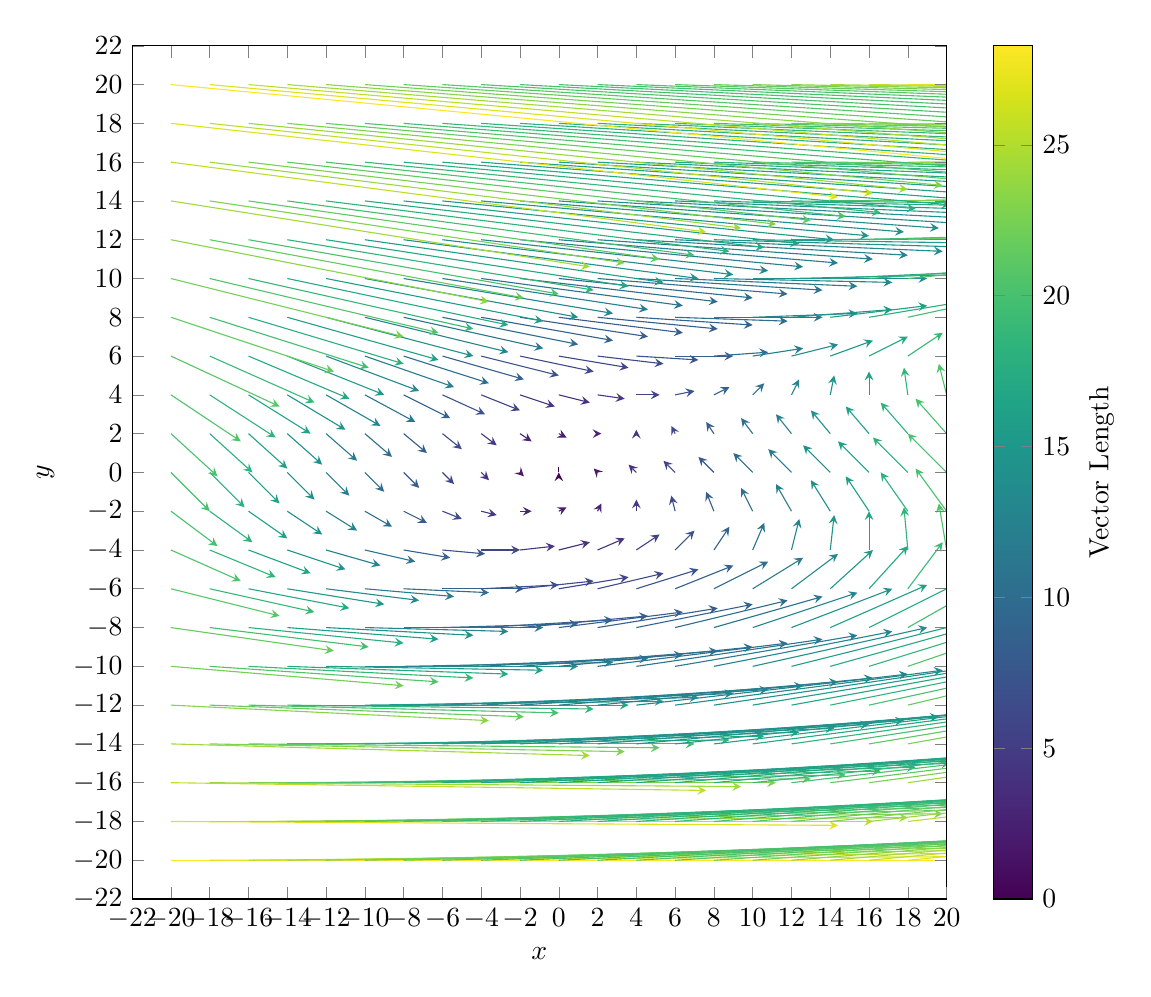
\begin{tikzpicture}
        \begin{axis}[
            xmin = -22, xmax = 20 ,
            ymin = -22, ymax = 22,
            zmin = 0, zmax = 1,
            axis equal image,
            xtick distance = 2,
            ytick distance = 2,
            view = {0}{90}, 
            scale = 2,
            %title = {\bf Vector Field $F = [-y,x]$},
            height=7cm,
            xlabel = {$x$},
            ylabel = {$y$},
            colormap/viridis,
            colorbar,
            colorbar style = {
                ylabel = {Vector Length}
            }
        ]
            \addplot3[
                point meta = {sqrt(x^2+y^2)},
                quiver = {
                    u = {-x+(-y)^2},
                    v = {-y+x}, 
                    scale arrows = 0.1,
                },
                samples=21,
                quiver/colored = {mapped color},
                -stealth,
                domain = -20:20,
                domain y = -20:20,
            ] {0};
        \end{axis}
    \end{tikzpicture}
\end{document}